\section{Experiment 1}
In this experiment we would like to experimentally verify how big time steps we can take before the simulation breaks down. As the simulation breaks down if the triangles collapse we need to ensure our time steps are small enough that the nodal velocities will not move the vertices 'through' an edge in the mesh. That is, in a single time step, no vertex should because of its velocity be moved beyond another vertex and collapse a triangle in the mesh. In \autoref{collapse} we see a vertex with a velocity, and if the time step is big enough the vertex will be moved 'to the outside' of the triangle. 
\begin{figure}
	\centering
	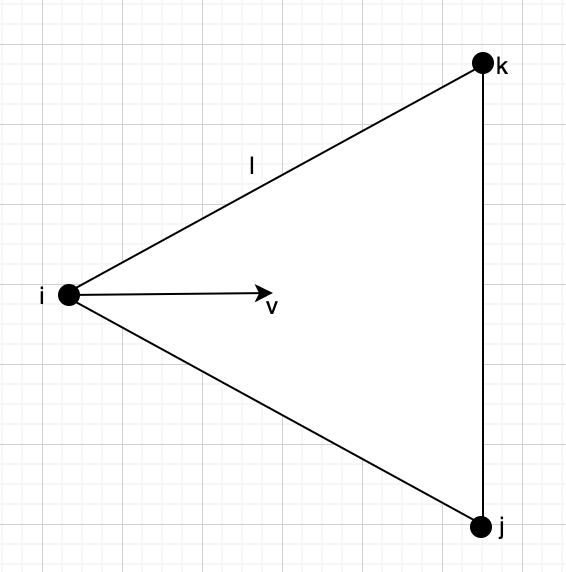
\includegraphics[width=0.55\linewidth]{Materials/collapse}
	\caption{A vertex \textit{i} with some velocity. If the time step we take gets too big, the vertex will be moved 'outside' the triangle, and the mesh will collapse.}
	\label{collapse}
\end{figure}
As it can be hard to measure the length the vertex has to travel before the triangle collapses, and we want this to hold for all vertices, we can approximate the length with the smallest edge length in the mesh. We can thus write the following relation:
\begin{align*}
	l_{min} &> \mathbf{v}_{max}\cdot \Delta t \iff \\
	\Delta t &< \frac{l_{min}}{\mathbf{v}_{max}}
\end{align*}
We can now look at our velocity update given by the Finite Volume Method derivation. The forces acting are primarily the elastic forces, and we simplify and only look at these:
\begin{equation*}
	\mathbf{v}^{t+\Delta t}_i = \mathbf{v}^t_i + \frac{\Delta t}{m_i}\mathbf{f}^{elastic}_i
\end{equation*}
We can here define the mass as $m_i = \rho l$. We also note from the derivation of the first Piola-Kirchhoff tensor, the second Piola-Kirchhoff tensor and the Green strain tensor that the Green strain tensor depend on the deformation gradient, and from the definition of the second Piola-Kirchhoff tensor we see $\lambda, \mu \propto \mathbf{E}$. As the lamé coefficients are proportional to Young's modulus, \textit{E}, we have $\mathbf{f}^{elastic}_i$ is proportional to Young's modulus, and thus we can substitute Young's modulus into our previous equation and find:
\begin{equation*}
	\mathbf{v}_{max} \propto \frac{\Delta t}{\delta l}E
\end{equation*}
Substituting this into our original relation we find:
\begin{align*}
	\Delta t &< \frac{l_{min}}{\mathbf{v}_{max}} \iff\\
	\Delta t &< \frac{l_{min}}{\frac{\Delta t}{\rho l_{min}}E} \iff\\
	\Delta t &< \frac{\rho l_{min}^2}{\Delta t E} \iff\\
	\Delta t &< \sqrt{\frac{\rho l_{min}^2}{E}}
\end{align*}
And we thus have an approximation to an upper bound on $\Delta t$. We can now run a series of experiments where we for different material find the largest $\Delta t$ where the simulation does not break down, and compare this with out analytically computed upper bound. Here we denote a successful simulation (a 'non-breakdown') as a simulation which runs for 1 second without showing unexpected behaviour. We use the same ball for the free fall for all materials, and the shortest edge in the ball is $0.080$. The results can be seen in \autoref{deltats}.
\begin{table}
	\centering
	\begin{tabular}{|c|c|c|c|c|}
		\hline
		Materials: & Rubber & Glass & Steel & concrete\\
		\hline
		$\Delta t$ used: & 0.00026 & 0.0000159 & 0.00001305 & 0.0000205\\
		\hline
		Upper bound: & 0.00082 & 0.000017 & 0.000016 & 0.000022\\
		\hline
		$\frac{\Delta t \text{used}}{\text{Upper bound}}$ & 0.317 & 0.935 & 0.816 & 0.931 \\
		\hline
	\end{tabular}
	\caption{Results of experiment 1.}
	\label{deltats}
\end{table}

\subsection{Discussion of results}
From our results we see that our upper bound does indeed hold for a wide arrange of materials. However, it does vary a little how tight of an upper bound it is. We here especially note how the upper bound for rubber is a lot higher than the $\Delta t$ actually used to make the simulation work. This is probably due to how much smaller Young's modulus is for rubber compared to the other materials used in the experiment, where the upper bound is a lot tighter. We thus conclude we have experimentally verified that we can find an upper bound to $\Delta t$ with the relation $\Delta t < C\sqrt{\frac{\rho l_{min}^2}{E}}$ where \textit{C} is a constant somewhere between $0.3$ and $0.9$.